\section{Entraînement du modèle}%
\label{sec.results.training}

Tous les tests présentés dans le reste de ce chapitre ont été effectués sur un ordinateur portable 
équipé d'un processeur \verb|Intel Core i9-8950HK| et d'une carte graphique \verb|NVIDIA GeForce GTX 1050 Ti|.
Cette machine se dispose de 32 Go de mémoire vive et de 4 Go de mémoire vidéo.
Le système d'exploitation est \verb|Ubuntu 20.04 LTS| et la version de Python utilisée est \verb|3.10.6|.


\subsection{Choix des hyperparamètres}%
\label{sub.results.training.hyperparameters}

Pour notre premier test, nous avons entraîné le modèle pour 20 époques.
Les hyperparamètres ont été choisis comme suit :
\begin{itemize}
    \item Dimension de plongement : 64
    \item Dimension de la couche cachée : 64
    \item Taux d'apprentissage : \(3 \times 10^{-4}\)
    \item Dropout : 0.1
    \item Nombre de couches de l'encodeur/décodeur : 3
    \item Nombre de têtes d'attention : 4
    \item Taille de lot : 256
    \item Nombre de processus pour le chargement des données : 4
\end{itemize}


\subsection{Résultats}%
\label{sub.results.training.results}

Pour chaque époque, nous avons calculé la moyenne de la fonction de perte, de l'exactitude et du score \gls{bleu} 
sur le corpus de validation et sur le corpus d'entraînement.
Les résultats sont présentés dans la Figure~\ref{fig.results.training}.
\begin{figure}[hbt]
    \begin{subfigure}{.5\textwidth}
        \begin{center}
            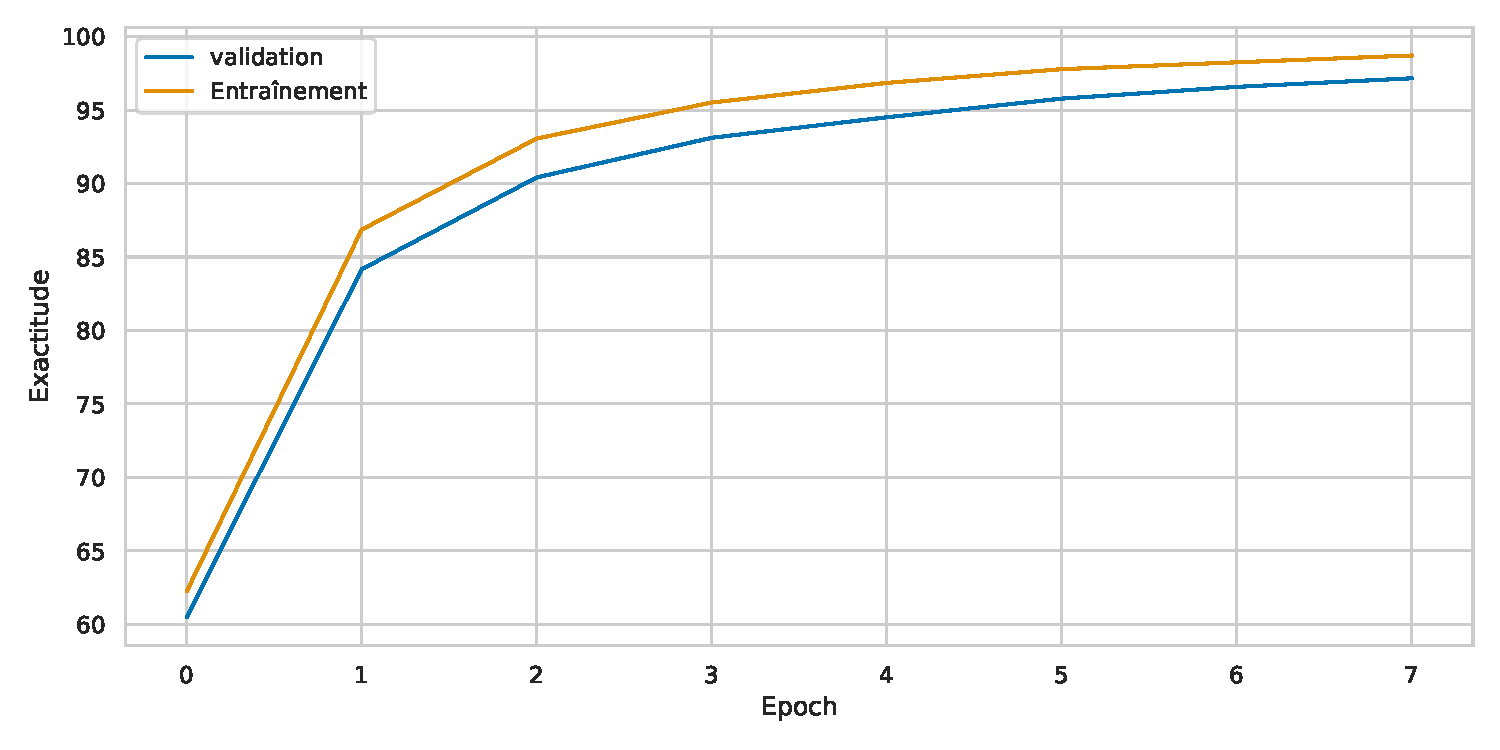
\includegraphics[width=\textwidth]{assets/python/accuracy.pdf}
        \end{center}
        \caption{Exactitude}
        \label{fig.results.training.accuracy}
    \end{subfigure}
    \begin{subfigure}{.5\textwidth}
        \begin{center}
            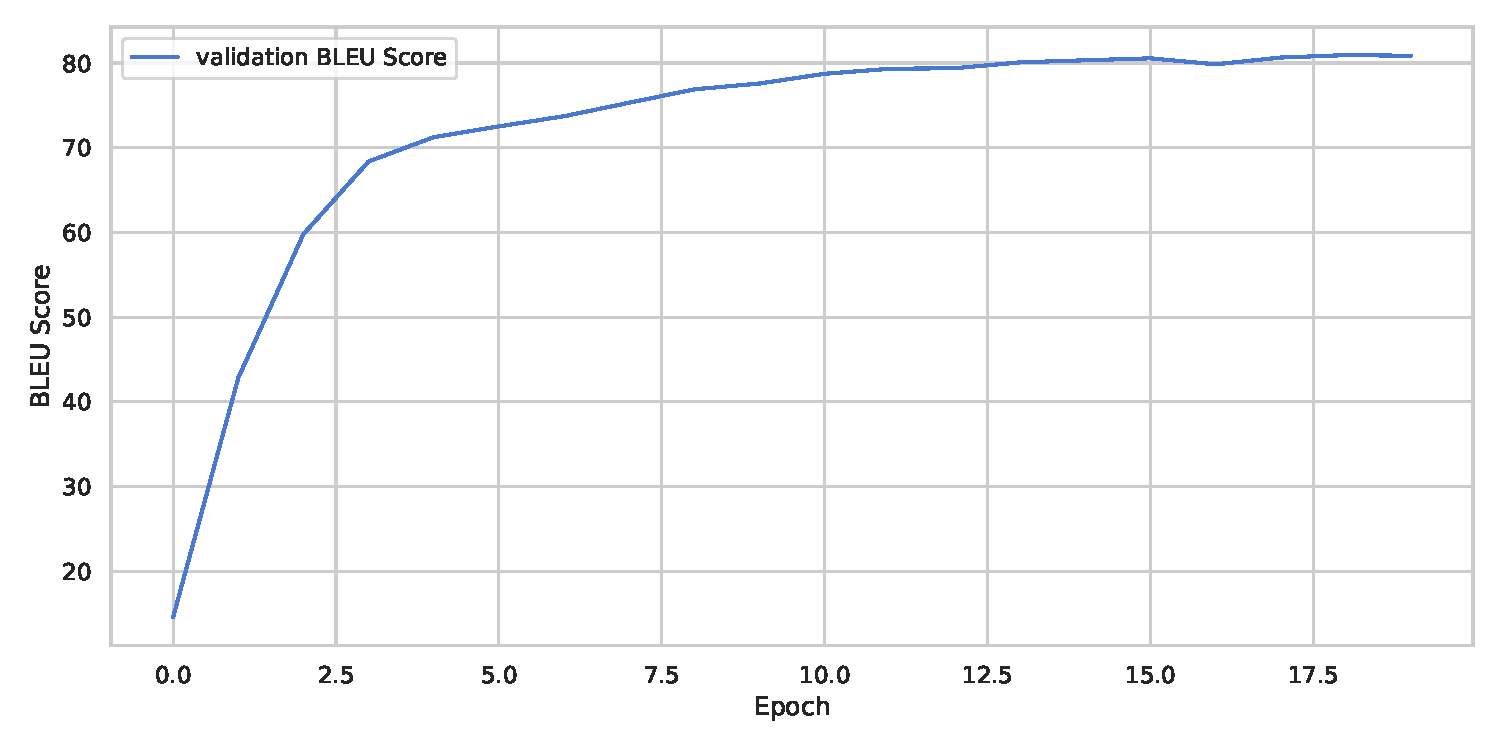
\includegraphics[width=\textwidth]{assets/python/bleu.pdf}
        \end{center}
        \caption{\glsfmtshort{bleu}}
        \label{fig.results.training.bleu}
    \end{subfigure}
    \begin{subfigure}{.5\textwidth}
        \begin{center}
            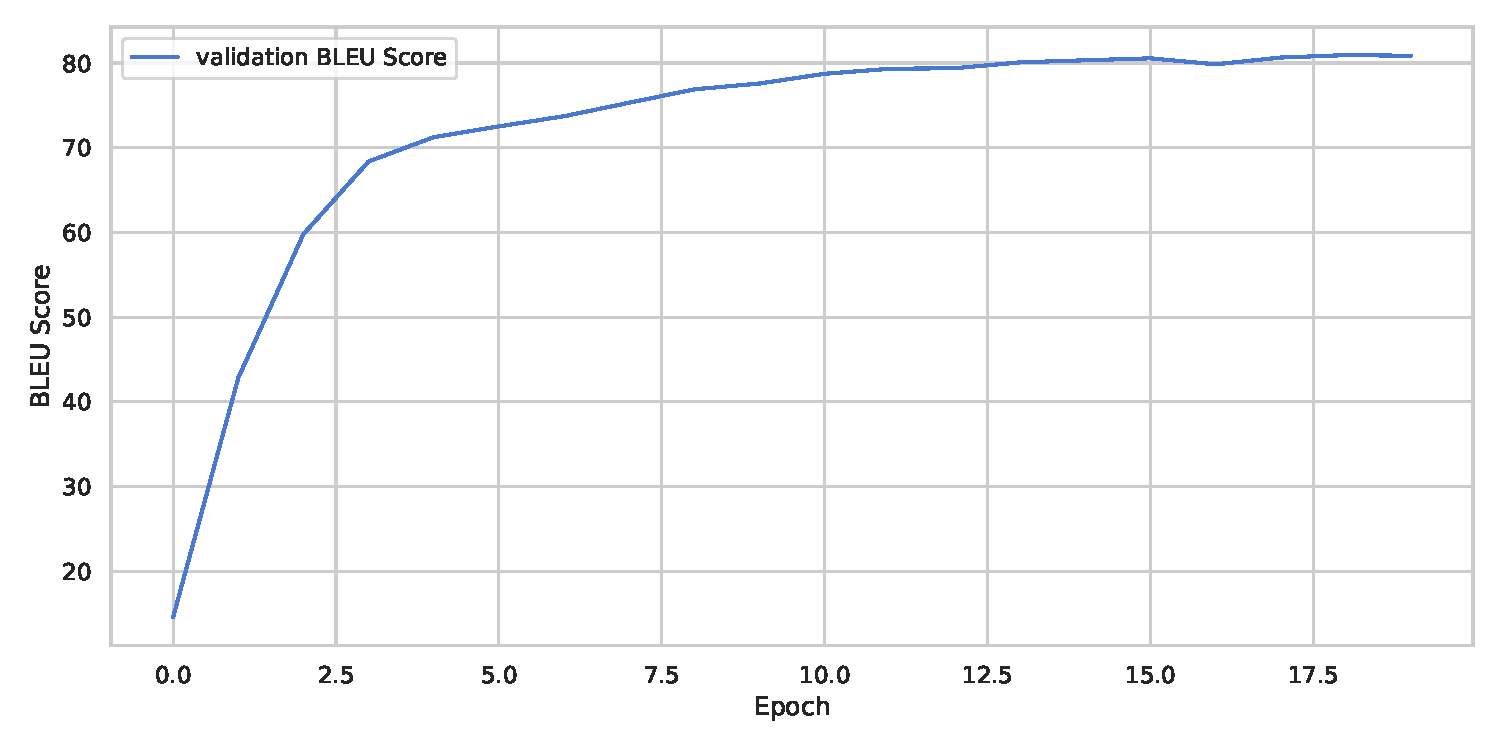
\includegraphics[width=\textwidth]{assets/python/bleu.pdf}
        \end{center}
        \caption{Perte}
        \label{fig.results.training.loss}
    \end{subfigure}
    \caption{Évolution des métriques au cours de l'entraînement.}
    \label{fig.results.training}
\end{figure}
Ces résultats sont satisfaisants.
Il n'est donc pas strictement nécessaire d'effectuer un réglage des hyperparamètres.
Cependant, il est possible en le faisant d'obtenir des résultats comparables 
en moins d'époques ou avec un modèle plus petit.
Pour cette raison, nous avons décidé de l'entamer.